% questions.tex —— 2003 年·北京卷·理科 · 题目内容片段（无答案）
% 由 tools/generate_projects.py 依来源总账自 2003/2003_数学真题_北京理_试题.md 生成，勿手改（改源 MD 后重跑）


\begin{gktip}
\textbf{来源说明}：本稿按固定候选 PDF 第 1–2 页逐题转录，原卷印刷页码 124–125。来源发布者、版次、复制/扫描链及官方身份未核。固定 PDF 仅含题面，无答案或评分页，官方答案字段为 null。
\textbf{题号范围}：原页可见 Q1–Q20；本候选 PDF 未见 Q21、Q22，不从其他版本补题。
\textbf{待核保留}：Q17 原页字面“底面边长的 3”未见“为”，照录并标记待核；不以语义补字。
\end{gktip}

\gkpart{一、选择题}

\begin{question}
\gkti{1}设集合
\nopagebreak[4]
\[
   A=\{x\mid x^2-1>0\},\qquad B=\{x\mid \log_2x>0\},
\]
   \((A\cap B)\) 等于\mbox{（　　）}

   (A) \(\{x\mid x>1\}\)　　(B) \(\{x\mid x>0\}\)

   (C) \(\{x\mid x<-1\}\)　　(D) \(\{x\mid x<-1\text{ 或 }x>1\}\)

\end{question}
\begin{question}
\gkti{2}设
\nopagebreak[4]
\[
   y_1=4^{0.9},\qquad y_2=8^{0.44},\qquad y_3=\left(\frac12\right)^{-1.5},
\]
   则\mbox{（　　）}

   (A) \(y_3>y_1>y_2\)　　(B) \(y_2>y_1>y_3\)

   (C) \(y_1>y_2>y_3\)　　(D) \(y_1>y_3>y_2\)

\end{question}
\begin{question}
\gkti{3}“\(\cos 2\alpha=-\dfrac{\sqrt3}{2}\)”是“\(\alpha=k\pi+\dfrac{5\pi}{12},\ k\in\mathbb Z\)”的\mbox{（　　）}

   (A) 必要非充分条件　　(B) 充分非必要条件

   (C) 充分必要条件　　(D) 既非充分又非必要条件

\end{question}
\begin{question}
\gkti{4}已知 \(\alpha,\beta\) 是平面，\(m,n\) 是直线。下列命题中不正确的是\mbox{（　　）}

   (A) 若 \(m\parallel n,\ m\perp\alpha\)，则 \(n\perp\alpha\)

   (B) 若 \(m\parallel\alpha,\ \alpha\cap\beta=n\)，则 \(m\parallel n\)

   (C) 若 \(m\perp\alpha,\ m\perp\beta\)，则 \(\alpha\parallel\beta\)

   (D) 若 \(m\perp\alpha,\ m\subset\beta\)，则 \(\alpha\perp\beta\)

\end{question}
\begin{question}
\gkti{5}极坐标方程
\nopagebreak[4]
\[
   \rho^2\cos 2\theta-2\rho\cos\theta=1
\]
   表示的曲线是\mbox{（　　）}

   (A) 圆　　(B) 椭圆　　(C) 抛物线　　(D) 双曲线

\end{question}
\begin{question}
\gkti{6}若 \(z\in\mathbb C\) 且 \(|z+2-2i|=1\)，则 \(|z-2-2i|\) 的最小值是\mbox{（　　）}

   (A) 2　　(B) 3　　(C) 4　　(D) 5

\end{question}
\begin{question}
\gkti{7}如果圆台的母线与底面成 \(60^\circ\) 角，那么这个圆台的侧面积与轴截面面积的比为\mbox{（　　）}

   (A) \(2\pi\)　　(B) \(\dfrac{3}{2}\pi\)　　(C) \(\dfrac{2\sqrt3}{3}\pi\)　　(D) \(\dfrac12\pi\)

\end{question}
\begin{question}
\gkti{8}从黄瓜、白菜、油菜、扁豆 4 种蔬菜品种中选出 3 种，分别种在不同土质的三块土地上，其中黄瓜必须种植，不同的种植方法共有\mbox{（　　）}

   (A) 24 种　　(B) 18 种　　(C) 12 种　　(D) 6 种

\end{question}
\begin{question}
\gkti{9}若数列 \(\{a_n\}\) 的通项公式是
\nopagebreak[4]
\[
   a_n=\frac{3^{-n}+2^{-n}+(-1)^n(3^{-n}-2^{-n})}{2},\qquad n=1,2,\ldots,
\]
   则 \(\displaystyle\lim_{n\to\infty}(a_1+a_2+\cdots+a_n)\) 等于\mbox{（　　）}

   (A) \(\dfrac{11}{24}\)　　(B) \(\dfrac{17}{24}\)　　(C) \(\dfrac{19}{24}\)　　(D) \(\dfrac{25}{24}\)

\end{question}
\begin{question}
\gkti{10}某班试用电子投票系统选举班干部候选人。全班 \(k\) 名同学都有选举权和被选举权，他们的编号分别为 \(1,2,\ldots,k\)。规定：同意按“1”，不同意（含弃权）按“0”，令
\nopagebreak[4]
\[
    a_{ij}=\begin{cases}
    1,&\text{第 }i\text{ 号同学同意第 }j\text{ 号同学当选},\\
    0,&\text{第 }i\text{ 号同学不同意第 }j\text{ 号同学当选},
    \end{cases}
\]
    其中 \(i=1,2,\ldots,k\)，且 \(j=1,2,\ldots,k\)，则同时同意第 1、2 号同学当选的人数为\mbox{（　　）}

    (A) \(a_{11}+a_{12}+\cdots+a_{1k}+a_{21}+a_{22}+\cdots+a_{2k}\)

    (B) \(a_{11}+a_{21}+\cdots+a_{k1}+a_{12}+a_{22}+\cdots+a_{k2}\)

    (C) \(a_{11}a_{12}+a_{21}a_{22}+\cdots+a_{k1}a_{k2}\)

    (D) \(a_{11}a_{21}+a_{12}a_{22}+\cdots+a_{1k}a_{2k}\)

\end{question}
\gkpart{二、填空题}

\begin{question}
\gkti{11}函数
\nopagebreak[4]
\[
    f(x)=\lg(1+x^2),\qquad
    g(x)=\begin{cases}
    x+2,&x<-1,\\
    0,&|x|\le 1,\\
    -x+2,&x>1,
    \end{cases}
    \qquad h(x)=\tan 2x
\]
    中，\gkblank{} 是偶函数。

\end{question}
\begin{question}
\gkti{12}以双曲线
\nopagebreak[4]
\[
    \frac{x^2}{16}-\frac{y^2}{9}=1
\]
    右顶点为顶点、左焦点为焦点的抛物线的方程是\gkblank{}。

\Needspace{0.4\textheight}
\end{question}
\begin{question}
\gkti{13}如图，已知底面半径为 \(r\) 的圆柱被一个平面所截，剩下部分母线长的最大值为 \(a\)，最小值为 \(b\)，那么圆柱被截后剩下部分的体积是\gkblank{}。
\nopagebreak[4]
\begin{center}% Generator: hand-authored TikZ schematic traced from the fixed source; cylinder proportions are illustrative.
% Source ID: src-120ea104f8cb373f5731039fa9d36469df457869849f27420831962ef1ad2306
% PDF SHA-256: d0081500bd56d03199ddcf232fe8e870f2ecd7e9c41ba849417af9af79fbb702
% PDF page 1; printed page 124; question 13.
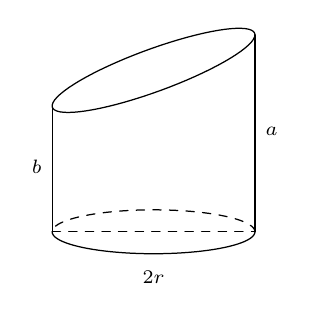
\begin{tikzpicture}[
  x=0.92cm,y=0.82cm,line width=0.45pt,line cap=round,
  every node/.style={font=\scriptsize,inner sep=1.5pt}
]
  % Lower base: dashed rear arc and diameter, solid front arc.
  \draw[dashed,domain=0:180,samples=48,variable=\t]
    plot ({1.4*cos(\t)},{0.34*sin(\t)});
  \draw[domain=180:360,samples=48,variable=\t]
    plot ({1.4*cos(\t)},{0.34*sin(\t)});
  \draw[dashed] (-1.4,0)--(1.4,0);

  % Oblique cut ellipse: the right generator is longer than the left one.
  \draw[domain=0:360,samples=72,variable=\t]
    plot ({1.4*cos(\t)},{2.5+0.55*cos(\t)+0.35*sin(\t)});
  \draw (-1.4,0)--(-1.4,1.95) (1.4,0)--(1.4,3.05);

  \node[left] at (-1.48,1.0) {$b$};
  \node[right] at (1.48,1.55) {$a$};
  \node[below] at (0,-0.54) {$2r$};
\end{tikzpicture}
\end{center}
\nopagebreak[4]
\end{question}
\begin{question}
\gkti{14}将长度为 1 的铁丝分成两段，分别围成一个正方形和一个圆形，要使正方形与圆的面积之和最小，正方形的周长应为\gkblank{}。

\end{question}
\gkpart{三、解答题}

\begin{question}
\gkti{15}已知函数
\nopagebreak[4]
\[
    f(x)=\cos^4x-2\sin x\cos x-\sin^4x.
\]

    (1) 求 \(f(x)\) 的最小正周期；

    (2) 若 \(x\in\left[0,\dfrac{\pi}{2}\right]\)，求 \(f(x)\) 的最大值、最小值。

\end{question}
\begin{question}
\gkti{16}已知数列 \(\{a_n\}\) 是等差数列，且 \(a_1=2,\ a_1+a_2+a_3=12\)。

    (1) 求数列 \(\{a_n\}\) 的通项公式；

    (2) 令 \(b_n=a_nx^n\ (x\in\mathbb R)\)。求数列 \(\{b_n\}\) 前 \(n\) 项和的公式。

\Needspace{0.4\textheight}
\end{question}
\begin{question}
\gkti{17}如图，正三棱柱 \(ABC-A_1B_1C_1\) 的底面边长的 3，侧棱 \(AA_1=\dfrac{3\sqrt3}{2}\)，\(D\) 是 \(CB\) 延长线上一点，且 \(BD=BC\)。

\begin{gktip}
原页疑点（待核）：原页可见字面为“底面边长的 3”，语句不完整，未见“为”；本稿照录，不按语义补字。
\end{gktip}

    (1) 求证：直线 \(BC_1\parallel\) 平面 \(AB_1D\)；

    (2) 求二面角 \(B_1-AD-B\) 的大小；

    (3) 求三棱锥 \(C_1-ABB_1\) 的体积。
\nopagebreak[4]
\begin{center}% Generator: hand-authored TikZ schematic traced from source-visible edges and labels; projection is illustrative.
% Source ID: src-120ea104f8cb373f5731039fa9d36469df457869849f27420831962ef1ad2306
% PDF SHA-256: d0081500bd56d03199ddcf232fe8e870f2ecd7e9c41ba849417af9af79fbb702
% PDF page 1; printed page 124; question 17.
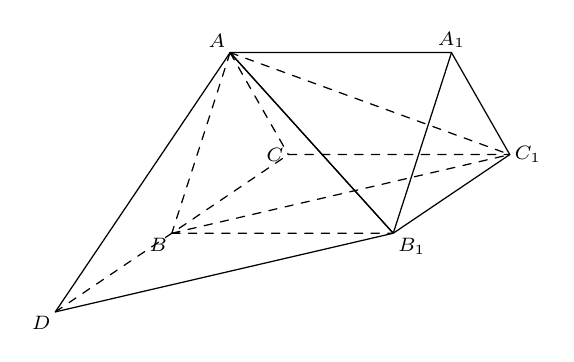
\begin{tikzpicture}[
  x=0.74cm,y=0.74cm,line width=0.45pt,line cap=round,line join=round,
  every node/.style={font=\scriptsize,inner sep=1.5pt}
]
  \coordinate (A)  at (0.7,4.2);
  \coordinate (A1) at (4.5,4.2);
  \coordinate (B)  at (-0.3,1.1);
  \coordinate (B1) at (3.5,1.1);
  \coordinate (C)  at (1.7,2.45);
  \coordinate (C1) at (5.5,2.45);
  \coordinate (D)  at (-2.3,-0.25);

  % Source-visible prism and auxiliary edges.
  \draw (D)--(A) (D)--(B1) (A)--(B1);
  \draw (A)--(A1)--(C1)--(B1)--cycle;
  \draw (A1)--(B1);
  \draw[dashed] (D)--(B)--(C) (A)--(B) (A)--(C);
  \draw[dashed] (A)--(C1) (B)--(B1) (B)--(C1) (C)--(C1);

  \node[above left] at (A) {$A$};
  \node[above] at (A1) {$A_1$};
  \node[below left] at (B) {$B$};
  \node[below right] at (B1) {$B_1$};
  \node[left] at (C) {$C$};
  \node[right] at (C1) {$C_1$};
  \node[below left] at (D) {$D$};
\end{tikzpicture}
\end{center}
\nopagebreak[4]
\Needspace{0.4\textheight}
\end{question}
\begin{question}
\gkti{18}如图，椭圆的长轴 \(A_1A_2\) 与 \(x\) 轴平行，短轴 \(B_1B_2\) 在 \(y\) 轴上，中心为 \(M(0,r)\)（\(b>r>0\)）。

    (1) 写出椭圆的方程，求椭圆的焦点坐标及离心率；

\Needspace{5\baselineskip}
    (2) 直线 \(y=k_1x\) 交椭圆于两点 \(C(x_1,y_1),D(x_2,y_2)\)（\(y_2>0\)）；直线 \(y=k_2x\) 交椭圆于两点 \(G(x_3,y_3),H(x_4,y_4)\)（\(y_4>0\)）。求证：
\nopagebreak[4]
\[
    \frac{k_1x_1x_2}{x_1+x_2}=\frac{k_2x_3x_4}{x_3+x_4};
\]

    (3) 对于 (2) 中的 \(C,D,G,H\)，设 \(CH\) 交 \(x\) 轴于点 \(P\)，\(GD\) 交 \(x\) 轴于点 \(Q\)。求证：\(|OP|=|OQ|\)。（证明过程不考虑 \(CH\) 或 \(GD\) 垂直于 \(x\) 轴的情形。）
\nopagebreak[4]
\begin{center}% Generator: hand-authored TikZ schematic traced from the fixed source; ellipse and chord coordinates are illustrative.
% Source ID: src-120ea104f8cb373f5731039fa9d36469df457869849f27420831962ef1ad2306
% PDF SHA-256: d0081500bd56d03199ddcf232fe8e870f2ecd7e9c41ba849417af9af79fbb702
% PDF page 2; printed page 125; question 18.
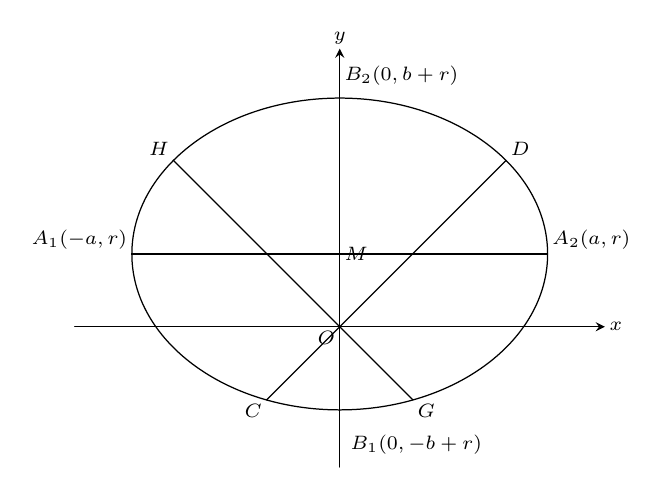
\begin{tikzpicture}[
  x=0.66cm,y=0.66cm,line width=0.45pt,line cap=round,>=stealth,
  every node/.style={font=\scriptsize,inner sep=1.5pt}
]
  \coordinate (O)  at (0,0);
  \coordinate (M)  at (0,1.4);
  \coordinate (A1) at (-4,1.4);
  \coordinate (A2) at (4,1.4);
  \coordinate (B1) at (0,-1.6);
  \coordinate (B2) at (0,4.4);
  \coordinate (H)  at (-3.2,3.2);
  \coordinate (G)  at (1.408,-1.408);
  \coordinate (C)  at (-1.408,-1.408);
  \coordinate (D)  at (3.2,3.2);

  \draw[->] (-5.1,0)--(5.1,0) node[right] {$x$};
  \draw[->] (0,-2.7)--(0,5.35) node[above] {$y$};
  \draw (M) ellipse [x radius=4,y radius=3];
  \draw (A1)--(A2);
  \draw (H)--(G) (C)--(D);

  \node[above left] at (A1) {$A_1(-a,r)$};
  \node[above right] at (A2) {$A_2(a,r)$};
  \node[above right] at (0,4.55) {$B_2(0,b+r)$};
  \node[below right] at (0.12,-2.0) {$B_1(0,-b+r)$};
  \node[right] at (M) {$M$};
  \node[below left] at (O) {$O$};
  \node[above left] at (H) {$H$};
  \node[below right] at (G) {$G$};
  \node[below left] at (C) {$C$};
  \node[above right] at (D) {$D$};
\end{tikzpicture}
\end{center}
\nopagebreak[4]
\Needspace{0.4\textheight}
\end{question}
\begin{question}
\gkti{19}有三个新兴城镇，分别位于 \(A,B,C\) 三点处，且 \(AB=AC=a,\ BC=2b\)。今计划合建一个中心医院，为同时方便三镇，准备建在 \(BC\) 的垂直平分线上的 \(P\) 点处。（建立坐标系如图）

    (1) 若希望点 \(P\) 到三镇距离的平方和为最小，点 \(P\) 应位于何处？

    (2) 若希望点 \(P\) 到三镇的最远距离为最小，点 \(P\) 应位于何处？
\nopagebreak[4]
\begin{center}% Generator: hand-authored TikZ schematic traced from the fixed source; triangle proportions are illustrative.
% Source ID: src-120ea104f8cb373f5731039fa9d36469df457869849f27420831962ef1ad2306
% PDF SHA-256: d0081500bd56d03199ddcf232fe8e870f2ecd7e9c41ba849417af9af79fbb702
% PDF page 2; printed page 125; question 19.
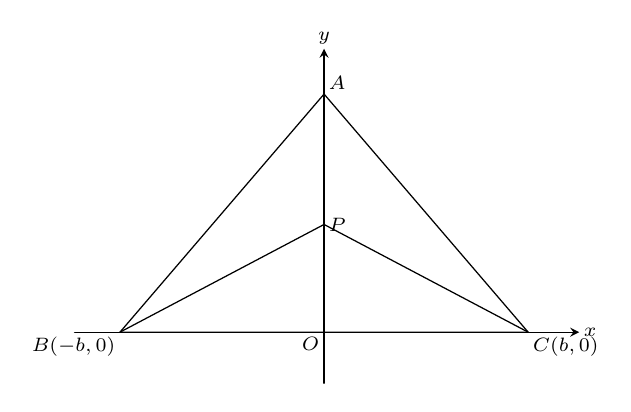
\begin{tikzpicture}[
  x=0.72cm,y=0.72cm,line width=0.45pt,line cap=round,>=stealth,
  every node/.style={font=\scriptsize,inner sep=1.5pt}
]
  \coordinate (O) at (0,0);
  \coordinate (A) at (0,4.2);
  \coordinate (P) at (0,1.9);
  \coordinate (B) at (-3.6,0);
  \coordinate (C) at (3.6,0);

  \draw[->] (-4.4,0)--(4.5,0) node[right] {$x$};
  \draw[->] (0,-0.9)--(0,5.0) node[above] {$y$};
  \draw (A)--(B)--(C)--cycle;
  \draw (P)--(B) (P)--(C);

  \node[above right] at (A) {$A$};
  \node[below left] at (B) {$B(-b,0)$};
  \node[below right] at (C) {$C(b,0)$};
  \node[below left] at (O) {$O$};
  \node[right] at (P) {$P$};
\end{tikzpicture}
\end{center}
\nopagebreak[4]
\end{question}
\begin{question}
\gkti{20}设 \(y=f(x)\) 是定义在区间 \([-1,1]\) 上的函数，且满足条件：

    ① \(f(-1)=f(1)=0\)；

    ② 对任意的 \(u,v\in[-1,1]\)，都有 \(|f(u)-f(v)|\le |u-v|\)。

    (1) 证明：对任意的 \(x\in[-1,1]\)，\(x-1\le f(x)\le 1-x\)；

    (2) 证明：对任意的 \(u,v\in[-1,1]\)，\(|f(u)-f(v)|\le 1\)；

\Needspace{5\baselineskip}
    (3) 在区间 \([-1,1]\) 上是否存在满足题设条件的奇函数 \(y=f(x)\)，且使得
\nopagebreak[4]
\[
    \begin{cases}
    |f(u)-f(v)|<|u-v|,&u,v\in\left[0,\dfrac12\right],\\
    |f(u)-f(v)|=|u-v|,&u,v\in\left[\dfrac12,1\right]?
    \end{cases}
\]
    若存在，请举一例；若不存在，请说明理由。

\end{question}